\documentclass[tikz,border=10pt]{standalone}
\usepackage{tkz-euclide} % 增强几何绘图工具
\usetikzlibrary{intersections, angles, quotes}

\begin{document}
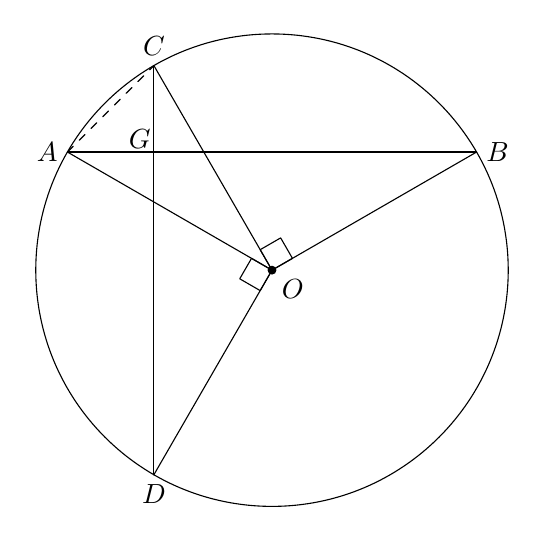
\begin{tikzpicture}[scale=2, line join=round, line cap=round, >=stealth]
    % 1. 定义基本参数（圆心与半径）
    \coordinate (O) at (0,0);
    \def\R{1.5}

    % 2. 定义关键点坐标 (基于图像几何关系提取)
    % A、C点通过角度定义，OA与OC垂直
    \coordinate (A) at (150:\R);
    \coordinate (C) at (120:\R);

    % 延长半径CO交圆于另一点D（即CD为直径，但图中D在下方）
    % 观察图：D点位于C点的对称位置附近。
    % 重新根据图示调整B和D的位置关系：
    % 观察到 OA ⊥ OC 且 OC ⊥ OB (直角符号)
    \coordinate (B) at (30:\R);  % OB ⊥ OC
    \coordinate (D) at (240:\R); % OD 为 OB 的反向延长线对称分布

    % 3. 绘制圆形
    \draw (O) circle (\R);

    % 4. 绘制连线
    \draw (A) -- (B);          % 弦 AB
    \draw (C) -- (D);          % 弦 CD
    \draw (O) -- (A) node[midway, below] {}; % 半径 OA
    \draw (O) -- (C);          % 半径 OC
    \draw (O) -- (B);          % 半径 OB
    \draw (O) -- (D);          % 半径 OD

    % 5. 绘制辅助线 (虚线 AC)
    \draw[dashed] (A) -- (C);

    % 6. 计算交点 G (AB 与 CD 的交点)
    \path[name path=lineAB] (A) -- (B);
    \path[name path=lineCD] (C) -- (D);
    \path[name intersections={of=lineAB and lineCD, by=G}];

    % 7. 绘制直角符号 (OA与OC垂直, OC与OB垂直)
    \tkzMarkRightAngle[size=0.15](A,O,D)
    \tkzMarkRightAngle[size=0.15](C,O,B)

    % 8. 绘制圆心点
    \fill (O) circle (0.8pt);

    % 9. 标注文本标签
    \node[left] at (A) {$A$};
    \node[right] at (B) {$B$};
    \node[above] at (C) {$C$};
    \node[below] at (D) {$D$};
    \node[below right] at (O) {$O$};
    \node[above left, inner sep=1pt] at (G) {$G$};

\end{tikzpicture}
\end{document}